\section{Aerosol Retrievals}

With the successful mission and relative radiance data from ALI the results need to be used to determine aerosol atmospheric parameters. The following sections will describe the MART retrieval method used, the results from using the MART method on the ALI data, and a comparison to the OSIRIS version 5.07 aerosol product and the from SALOMON a French gondola that flew before the CARMEN-2 gondola that measured aerosol extinction.

\subsection{Multiplicative Algebraic Reconstruction Technique}

In order to be able use the the measured radiances from ALI a forward model is needed to be able to determine the atmospheric state for a specific geometry given an atmospheric state. The SASKTRAN-HR polarized radiative transfer model \citep{Dueck2015} which was discussed in detail in \autoref{TODO:SASKTRAN}. This section focuses on the method used to solve the nonlinear inverse problem known as the Multiplicative Algebraic Reconstruction Technique (MART.)

The Multiplicative Algebraic Reconstruction Technique (MART) is a measurement inversion technique where a measured value can be converted into a wanted usable physical quantity via an iterative method. A measurement vector, $\mathbf{y}$, that has sensitivity to the desired physical state is constructed and is computed with a forward model, $F$ is used, in this case SASKTRAN, with an input state, $\mathbf{b}$, and a wanted parameter $\mathbf{x}$. The measurement vector is then calculated with the model and is yielded by
\begin{equation}
 \mathbf{y} = \mathbf{F}(\mathbf{x},\mathbf{b}) + \boldsymbol{\epsilon}
\end{equation}
where $\boldsymbol{\epsilon}$ is the noise on the measurement vector.

The MART was developed by \citep{Bourassa2012a} used with limb scatter instruments. An initial guess of the atmospheric state, $\mathbf{x}$ or a priori is assumed which is iteratively updated based on the ratio of the measured state, $\mathbf{y}$, to the forward model, $\mathbf{F}(\mathbf{x},\mathbf{b})$ and is computationally efficient as it allows for the updating of the atmospheric state without calculating the jacobian \cite{Degenstein2009}. This method is similar to the Chahine relaxation method \citep{Chahine1972} with the addition of a weighing matrix, $\mathbf{W_{ij}}$ which allows for relates the importance of each measurement vector to each shell altitude of the model, $i$ and the measured tangent altitude, $j$. The iterative method is given by
\begin{equation}
    x_{i}^{n+1} = x_{i}^{n}\sum_{j}\frac{y_{j}}{F_{i}(\mathbf{x},\mathbf{b})}W_{ij}.
\end{equation}
Now the formation of the measurement vectors is required in order to fins the atmospheric state but before the measurement vector can be discussed a description of the radiance is required.

\subsection{Measurement Vectors}

Now the formation of the measurement vectors is required in order to finds the atmospheric state but before the measurement vector can be discussed a description of the radiance is required. The polarized SASKTRAN-HR model gives the Stokes vectors for the radiance on its internal coordinate grid which can be retrieved from the model and then rotated to match ALI's coordinate system. Once rotated the polarization required to match ALI's measured results is the vertical polarization given by
\begin{equation}
    I = \frac{1}{2}\left(\mathrm{S_{0}}-\mathrm{S_{1}}\right)
\end{equation}
where $\mathrm{S_{0}}$ and $\mathrm{S_{1}}$ are Stokes parameters representing total radiance and horizontally polarized radiance respectively. From here on any reference to the radiance, $I$, in the rest of the chapter will refer to the vertical polarization measured by ALI.

The relative radiance level 1 data from ALI are used to create measurement vectors, $y$, in the following form
\begin{equation}
    \mathbf{y} = \log\left(\frac{\mathbf{I}(\mathbf{z},\lambda)}{I(z_{ref},\lambda)}\right)-\log\left(\frac{\mathbf{I}_{rayleigh}(\mathbf{z},\lambda)}{I_{rayleigh}(z_{ref},\lambda)}\right)
    \label{eqn:5.3:measurementVector}
\end{equation}
where $\mathbf{I}(\mathbf{z},\lambda)$ is the measured radiance from ALI and $I(z_{ref},\lambda)$ is the radiance at a reference altitude used to normalize the signal from a high altitude where there is little aerosol contribution, for ALI the highest possible altitude where the signal is above the noise threshold is around 25-30~km tangent height. The second term is modeled values from SASKTRAN-HR with only background neutral atmosphere to remove the rayleigh signal from the measured radiances which is done to improve the speed of the convergence of the retrieval. The left panel of \autoref{fig:5.3:measurementVectors} shows the measurement vector from a 750~nm image, number 208, from the 0\si{\degree} horizontal line of sight. The final measurement vector, $\mathbf{y}$ is shown in the black, with the first term of \autoref{eqn:5.3:measurementVector} is in blue and the second term is in red. The reason why removing the rayleigh component of the signal from the data increases the speed of the convergence of the solution is that most of the measured signal from ALI is comprised of the rayleigh component, in red, by removing the rayleigh component of the signal the resulting in a measurement vector just primarily sensitive to aerosol. The ALI measurement vector is similar to the measurement vector used for the OSIRIS retrieval \citep{Bourassa2007,Bourassa2011} and all of the the measurement vectors for the 750~nm 0\si{\degree} horizontal line of sight form the mission can be seen in the right of \autoref{fig:5.3:measurementVectors}.

The error for a measurement vector is required to be able to determine the error on the final retrieved aerosol profile. To yield this term \autoref{eqn:5.3:measurementVector} is differentiated giving the following result
\begin{equation}
    \delta\mathbf{y}^{2} = \left(\frac{\delta\mathbf{I}(\mathbf{z},\lambda)}{\mathbf{I}(\mathbf{z},\lambda)}\right)^{2} + \left(\frac{\delta I(z_{ref},\lambda)}{I(z_{ref},\lambda)}\right)^{2} + \left(\frac{\delta\mathbf{I}_{rayleigh}(\mathbf{z},\lambda)}{\mathbf{I}_{rayleigh}(\mathbf{z},\lambda)}\right)^{2} + \left(\frac{\delta I_{rayleigh}(z_{ref},\lambda)}{I_{rayleigh}(z_{ref},\lambda)}\right)^{2}.
\end{equation}
However, the only error considered is in the analysis is error due to the instrument, since the rayleigh component are modeled they are dropped from the error, simplifying the above result to
\begin{equation}
    \delta\mathbf{y}^{2} = \left(\frac{\delta\mathbf{I}(\mathbf{z},\lambda)}{\mathbf{I}(\mathbf{z},\lambda)}\right)^{2} + \left(\frac{\delta I(z_{ref},\lambda)}{I(z_{ref},\lambda)}\right)^{2}.
\end{equation}
An example of this error on the measurement vector on image 208 is located on the middle panel of \autoref{fig:5.3:measurementVectors}.

A similar measurement vector is used for the forward model except base aerosol state or a priori, $\mathbf{x}$, is assumed for aerosol extinction profile and the both terms of the expression is calculated by SASKTRAN yielding the following
\begin{equation}
    \mathbf{F}(\mathbf{x},\mathbf{b}) = \log\left(\frac{\mathbf{I}_{mod}(\mathbf{z},\lambda)}{I_{mod}(z_{ref},\lambda)}\right)-\log\left(\frac{\mathbf{I}_{rayleigh}(\mathbf{z},\lambda)}{I_{rayleigh}(z_{ref},\lambda)}\right)
    \label{eqn:5.3:forwardModel}
\end{equation}
where $\mathbf{I}_{mod}(\mathbf{z},\lambda)$ is the modeled radiance for the measurement and $I_{mod}(z_{ref},\lambda)$ is the measurement at the same reference altitude for normalization.

\begin{figure}
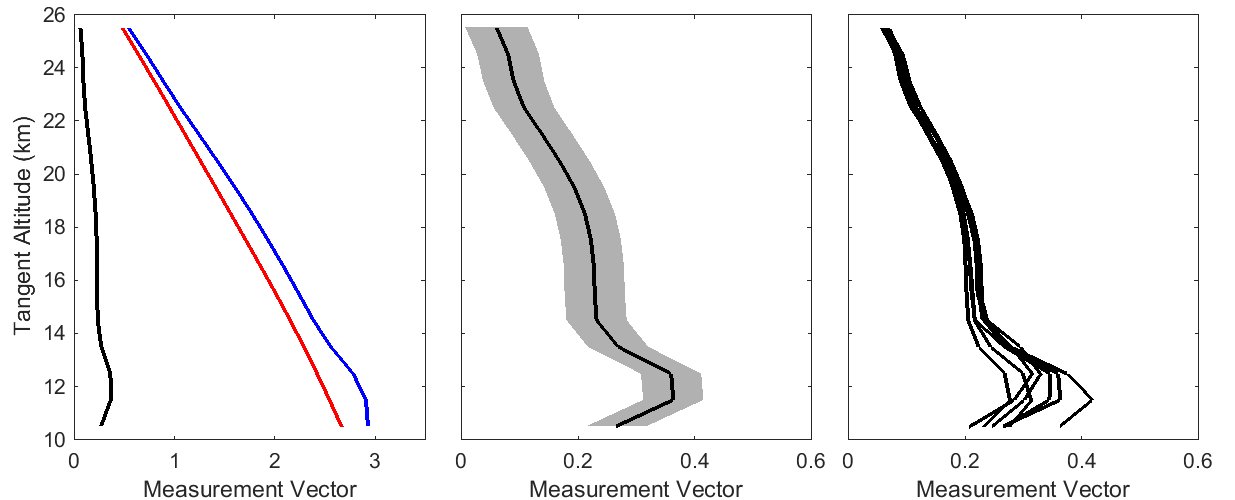
\includegraphics[width=1.0\textwidth]{./Images/5-3-MeasurementVectorsComparisons.pdf}
    \caption[ALI Measurement Vectors]{Left: The measurement vector and two corresponding terms for \autoref{eqn:5.3:measurementVector} of the 0\si{\degree} line of sight of image 208. The black, blue, red curves represent the measurement vector, first term of \autoref{eqn:5.3:measurementVector}, and second term of \autoref{eqn:5.3:measurementVector}. Middle: Image 208 0\si{\degree} line of sight measurement vector with associated error represented by the shading. Right: A collection of all of the 0\si{\degree} line of sight measurement vectors at 750~nm during the mission.}
    \label{fig:5.3:measurementVectors}
\end{figure}

\subsection{Retrieval and Results}

In order to be able to use the ALI measurement vectors in the MART method certain quantities were needed for the model; albedo, ozone concentration and cross sections, and aerosol cross sections. The albedo is required since an absolute radiance calibration was never preformed with ALI and the albedo cannot be determined directly from ALI's measurements, which is important since the amount of ground scatter in SASKTRAN-HR must correspond to the ground scatter during ALI's flight. Second, the ozone absorbtion features from the Chappuis band appear in the ALI measurements from 650 to 700~nm. The absorbtion must be accounted for to not artificially change the determined aerosol profiles. The ozone profiles were acquired from OSIRIS instrument using the five scans that were within 48 hours of the balloon flight and within 500~km of the launch facility were averaged together to be the ozone profile used in the SASKTRAN-HR model, with cross sections from \cite{Burrows1999}. The albedo is from the ADAM database which has monthly values for albedo over the surface on earth at a resolution of 0.1\si{\degree}~x~0.1\si{\degree} grid at 1~nm spectral resolution \citep{Muller2013}. The aerosol cross sections come from the Mie scattering derivation that was originally proposed by Mie and was implemented efficiently by \cite{Wiscombe1980}. For the purpose of the retrieval an a priori for particle was used with a mode radius of 0.08~$\si{\micro\metre}$  and a mode width of 1.6 in a log-normal distribution which is considered a standard size distribution for aerosol \citep{Deshler2003}.

The complete mission consisted of 216 images that were recorded in illuminated conditions. The MART retrieval method was run on a select set for the purpose of the analysis, specifically the last complete set of images from 650 to 950~nm consisting of images 204-216. They were chosen due to being the last in the mission and the sun was the highest in the sky giving the brightest atmosphere leading to the best signal to noise during the mission. A sample of the retrievals can be observed in \autoref{fig:5.3:AliRetreivals} which highlights the 725, 825, and 925~nm retrievals for images 206. The left panels shows the measurement vector from ALI in black with the forward model radiance profile from SASKTRAN-HR in blue. For each of the wavelengths, the algorithm determines altitudes where the value of the measurement vector is less than the known noise and does not allow aerosol to be retrieved in those regions. Instead the scaling factor, given by $\alpha = yF^{-1}$ is scaled to the aerosol profile above and below the last retrieved point to keep the aerosol profile smooth, as discontinuities are nonphysical and can lead to a nonphysical results in the MART algorithm. The middle panel shows the convergence between the measurement vector and the forward model result. For the full range of the wavelengths a difference of less than 1\% is seen from 12 to 24~km with a few outliers.

\begin{figure}
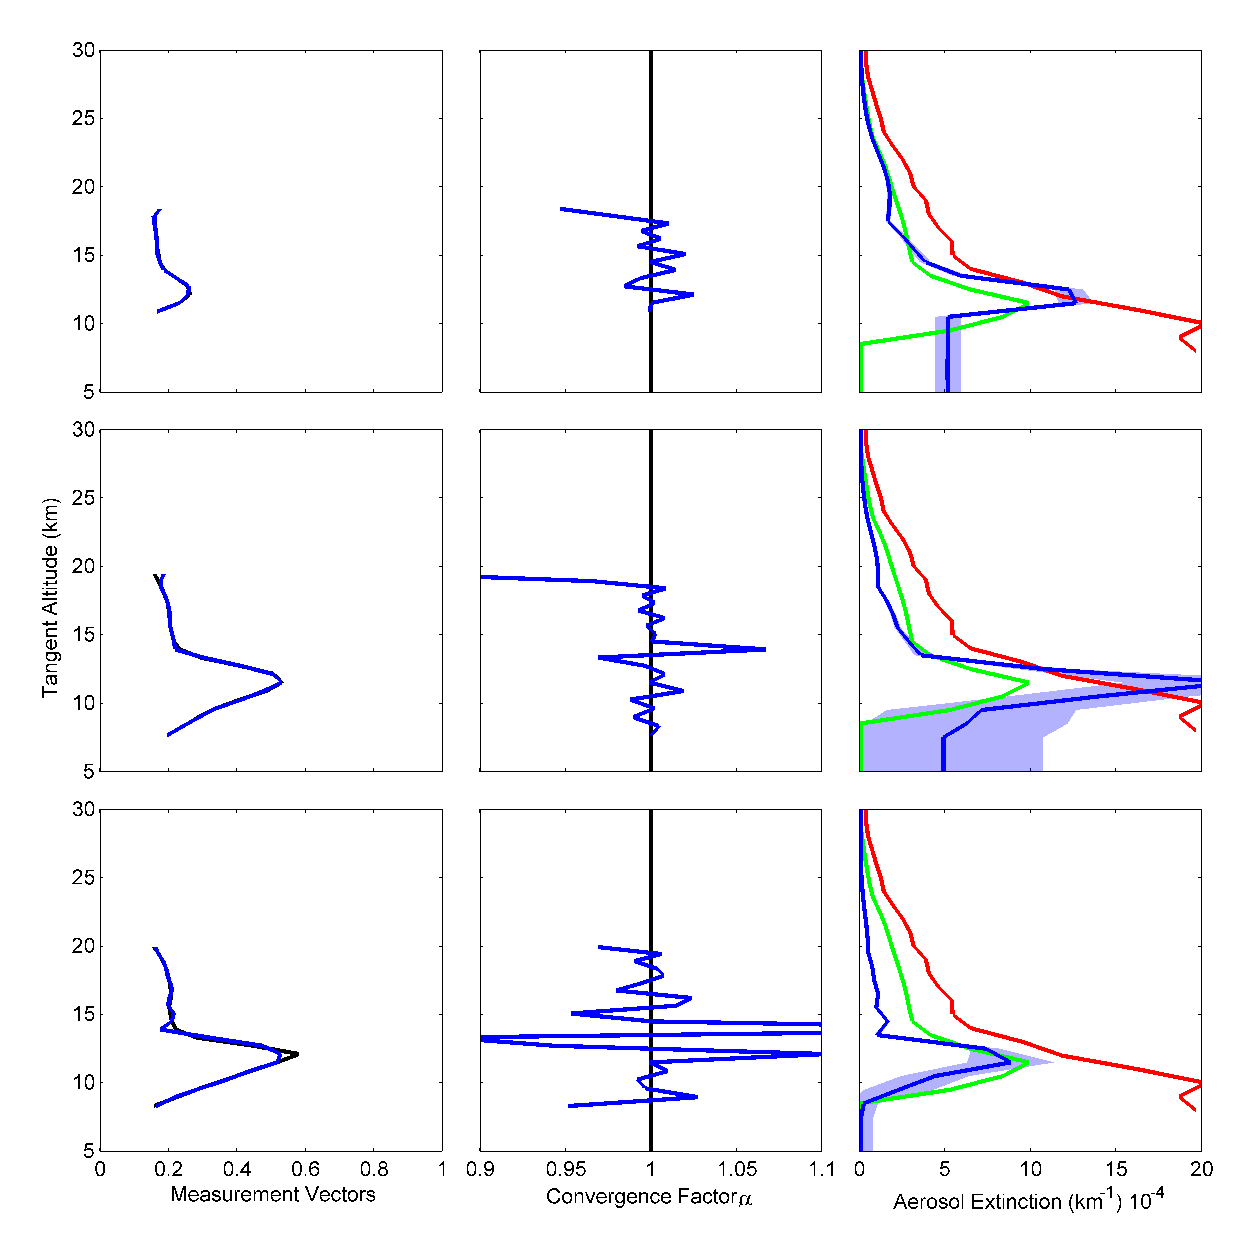
\includegraphics[width=1.0\textwidth]{./Images/5-3-AliRetreivals.pdf}
    \caption[ALI Aerosol Retrievals]{An example of three aerosol retrievals from images 206, 208, and 214, with center wavelengths of 700, 750, and 900~nm respectively vertically displayed in the figure from top to bottom. The left column shows the measurement vector, $y$, in black with the retrieved forward model, $F$, in blue. The center column shows the ratio of the $y$ over $F$ known as $\alpha$ and is the convergence factor between the ALI measurement and the forward model. For both the first two columns the black line is barely viable due to the very good agreement of the forward model. The final column is ALI aerosol extinction in blue with the associated error represented by the light blue shading.}
    \label{fig:5.3:AliRetreivals}
\end{figure}

The complete set of aerosol extinction profiles for the last cycle can be seen in the left panel of \autoref{fig:5.3:AliAerosolCycle} fromt he 0\si{\degree} horizontal line of sight. From the retrieval altitudes the aerosol extinctions do not show then expected decrease as the wavelength increases. The extinction is the number density multiplied by the scattering cross section, theoretically the number density should not change with respect to wavelength but the scattering cross section, according to Mie theory, should decrease with wavelength. However since a particle size distribution is assumed, and not determined, there will be a error associated with these extinctions and a method to determined particle size will be discussed in \autoref{sec:5.4:ParticleSizeDetermineation}.

With the successful aerosol retrieval from the mission the question that remains is how do these results compare to other aerosol extinction measuring instrument. Two other instruments are used to compare with the ALI results, the satellite based OSIRIS and stratospheric balloon based SALOMON. The ALI aerosol profile for the 750~nm aerosol extinction is shown in blue with the shading representing the error for the retrieval on the right of \autoref{fig:5.3:AliAerosolCycleNoPartSize}. The error is strictly based on measurement error and neglecting any model and atmospheric state errors. The green curve is the average 750~nm aerosol extinction profiles of the same five OSIRIS scans used for the ozone profile and OSIRIS uses a retrieval method for aerosol that is very similar to the method used for ALI \citep{Bourassa2007,Bourassa2011}. The red is the 750~nm aerosol extinction from SALOMON \citep{Berthet2002} which was balloon launched from the Timmins balloon base as the Nimbus 5 mission on September 12, 2014. The aerosol extinction for ALI and OSIRIS are within agreement of each other within the error for a majority of the 750~nm profile with some disagreement between 18 to 24~km. It also should be noted that the three instruments follow the same overall profile shape.  First, a bend in the profile occurs at approximately 25~km, then increases approximately linearly until 15~km where aerosol extinction leaves the linear trend and forms the peak of the measurement. The agreement in shape is an excellent result for the ALI mission since it shows good sensitivity to aerosol.

\begin{figure}
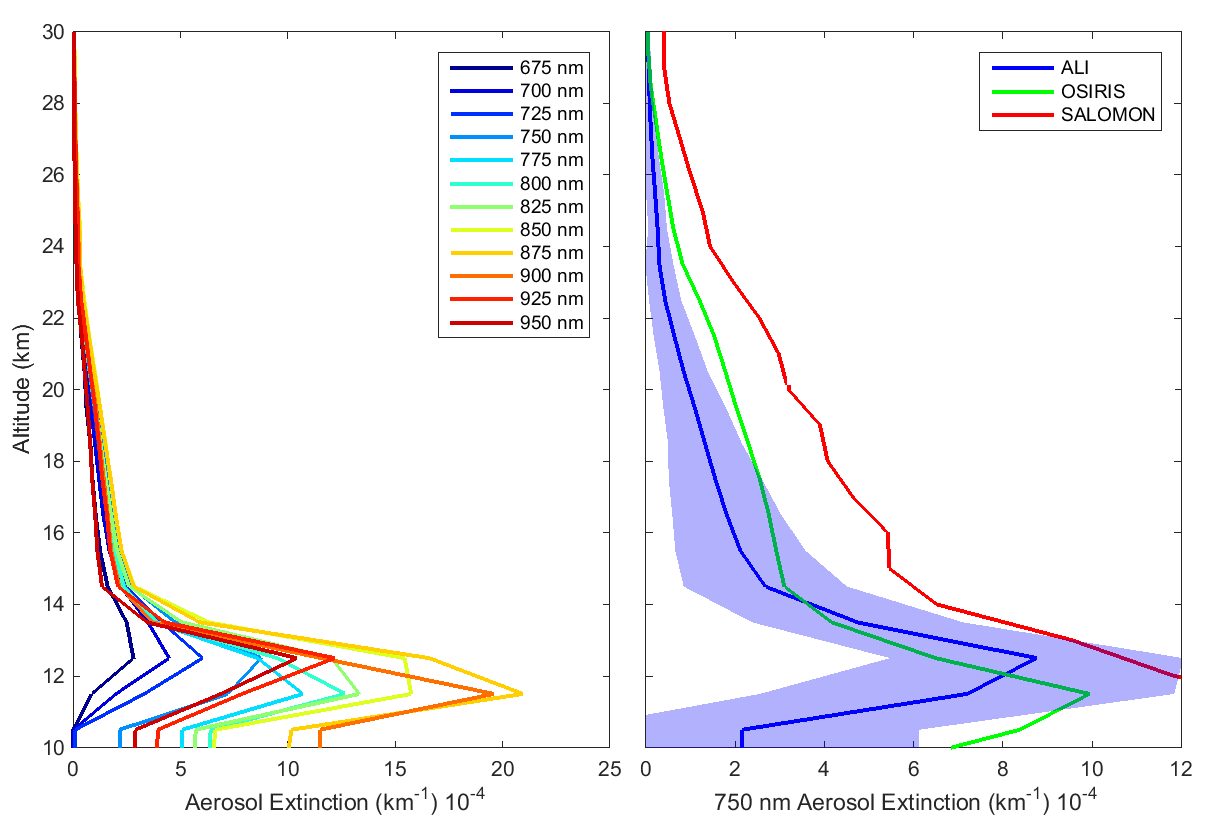
\includegraphics[width=1.0\textwidth]{./Images/5-3-FullAerosolCycleComparisonNoPartSize.pdf}
    \caption[Aerosol Retrievals for All Wavelengths and 750~nm Comparison with OSIRIS and SALOMON]{Left is the retrieved aerosol extinction profiles from the last complete cycle consisting of images 205 to 216 from the 0.0\si{\degree} horizontal line of sight. Right is the 750~nm ALI aerosol extinction in blue with its error represented by the shading compared to the 750~nm extinction measured by OSIRIS and SALOMON in green and red respectively.}
    \label{fig:5.3:AliAerosolCycleNoPartSize}
\end{figure}

As noted in \autoref{fig:5.3:AliAerosolCycleNoPartSize} an error was determined for the ALI retrievals and was determined in the following method. Start by preforming the retrieval on the measurement vector to yield the determined aerosol state. Next since iterative states always slightly change with additional iteration and need to be removed to not be considered part of the noise error on the analysis the aerosol profile is is reretrieved, $\mathbf{k}$. Then perturb the measurement vector at the first retrieved altitude and retretrieve the aerosol profile yielding $\mathbf{k}_{1}$, and create the first column of the error matrix, $\mathbf{E}$, by takeing $\delta\mathbf{k}_{1} = \mathbf{k}_{1}-\mathbf{k}$ which removed the initial profile plus the precision error from reretieveing the profile. Repeat for the rest of the retrieved altitudes, $n$, yielding the error matrix
\begin{equation}
    \mathbf{E} =
    \left[ \begin{array}{ccccc}
    \vdots & \vdots & \vdots & \vdots \\
    \delta\mathbf{k}_{1} & \delta\mathbf{k}_{2} & \dots & \delta\mathbf{k}_{n} \\
    \vdots & \vdots & \vdots & \vdots
    \end{array} \right].
\end{equation}
Each row is the error matrix is caused by a specific height of the retrieval, $j$, the total error on each profile height is given is given by
\begin{equation}
    \epsilon_{j} = \left( \sum^{m}_{i} E_{ij}^{2} \right)^{0.5}
\end{equation}
where $m$ is the total number of retrievals altitudes. Since the ALI measurements are normalized to a 1~km grid for ALI $\mathbf{E}$ is a square matrix.


%\egin{enumerate}
%    \item Preform the retrieval for the measurement vector in question and store the aerosol profile.
%    \item Repreform the retrieval with the new aerosol state and store the difference between the retrieved profile and the retrieved profile.
%    \item At each altitude perturb the measurement vector by the known error.
%    \item Reretieve the aerosol profile for the perturbed state and create a column in an precision matrix
%\end{enumerate}
%For the profile in question  An error estimation was also needed to be able to fully classify the capabilities of ALI and was performed using a perturbation method. Once a retrieval has been completed for an horizontal line of sight for an image the result is used to estimate the error in the returned extinction. For each altitude, the measurement vector is perturbed by the error resulting form the level 0 to level 1 data conversion parameters used and from the readout electronics. The MART retrieval is rerun and the change of the extinction is determined. These are compiled to form a gain matrix, $\mathbf{G}$, with size is $n$ by $m$ which are the shell altitudes and the tangent altitudes grids respectively, with elements $g_{ij}$. The error at each retired altitude is then given by
%\begin{equation}
%    e_{i} = \left(\sum_{j}g_{ij}g_{ji}\right)^{0.5}
%\end{equation}
%which gives the error at at retrieved altitud.e

